%-----------------------------------------------------------------------
%Copyright (c) 2011,  Ashish Tiwari.
%Developed with the sponsorship of the Defense Advanced Research Projects Agency (DARPA).
% 
%Permission is hereby granted, free of charge, to any person obtaining a copy of this data, including
%any software or models in source or binary form, as well as any drawings, specifications, and
%documentation (collectively "the Data"), to deal in the Data without restriction, including without
%limitation the rights to use, copy, modify, merge, publish, distribute, sublicense, and/or sell copies
%of the Data, and to permit persons to whom the Data is furnished to do so, subject to the following
%conditions:
%
%The above copyright notice and this permission notice shall be included in all copies or substantial
%portions of the Data.
%
%THE DATA IS PROVIDED "AS IS", WITHOUT WARRANTY OF ANY KIND, EXPRESS OR IMPLIED, INCLUDING BUT NOT
%LIMITED TO THE WARRANTIES OF MERCHANTABILITY, FITNESS FOR A PARTICULAR PURPOSE AND NONINFRINGEMENT. IN
%NO EVENT SHALL THE AUTHORS, SPONSORS, DEVELOPERS, CONTRIBUTORS, OR COPYRIGHT HOLDERS BE LIABLE FOR ANY
%CLAIM, DAMAGES OR OTHER LIABILITY, WHETHER IN AN ACTION OF CONTRACT, TORT OR OTHERWISE, ARISING FROM,
%OUT OF OR IN CONNECTION WITH THE DATA OR THE USE OR OTHER DEALINGS IN THE DATA.
%
\documentclass{seminar}
\usepackage{epic,/homes/tiwari/Talks/Special/relative,latexsym,url}
\usepackage{/homes/tiwari/Talks/Special/gastex}
\usepackage{wrapfig}

\usepackage{fancybox}
\usepackage{semlayer}
\usepackage{epsfig}
\usepackage{amssymb}
\usepackage{semcolor}

\def\printlandscape{\special{landscape}}    % Works with dvips.
\renewcommand{\printlandscape}{\special{landscape}}
\special{! /landplus90 true store}

\input{/homes/tiwari/Talks/Special/slideprel}
\slideframe{oval}
\usepackage{times} 		%% for PDF purposes

\newcommand\ignore[1]{{{}}}

% \ifpdf\else
%%%%%%%%
% to fix problems making landscape seminar pdfs
% Letter...
%\pdfpagewidth=11truein
%\pdfpageheight=8.5truein
% A4
\pdfpagewidth=297truemm % your milage may vary....
\pdfpageheight=210truemm
\pdfhorigin=1truein     % default value(?), but doesn't work without
\pdfvorigin=1truein     % default value(?), but doesn't work without
%\fi
% -------------------------------------------------------

%---------------------------------------------------------------------
\begin{document}
%---------------------------------------------------------------------
\begin{slide}
\heading{Powertrain Simulation Plots}

Included here are simulation plots generated using the
powertrain model for three different scenarios:

In all scenarios, car is moving on a road with constant
grade with the throttle at a constant position

\begin{description}
\item[Scenario 1]: tps = 10\%, grade = 0
\item[Scenario 2]: tps = 50\%, grade = 0.1 radians
\item[Scenario 3]: tps = 80\%, grade = 0.2 radians
\end{description}

The last scenario is simulated twice:
once with step size 0.001s, and then with step size 0.0005s.
The first two scenarios are simulated with step size 0.001s.

\end{slide}
%---------------------------------------------------------------------
\begin{slide}
\heading{Powertrain Simulation Plots: tps=10\%,grade=0}
\begin{tabular}{ccc}
Transmission Torque & Vehicle Speed & Gear
\\ \hline
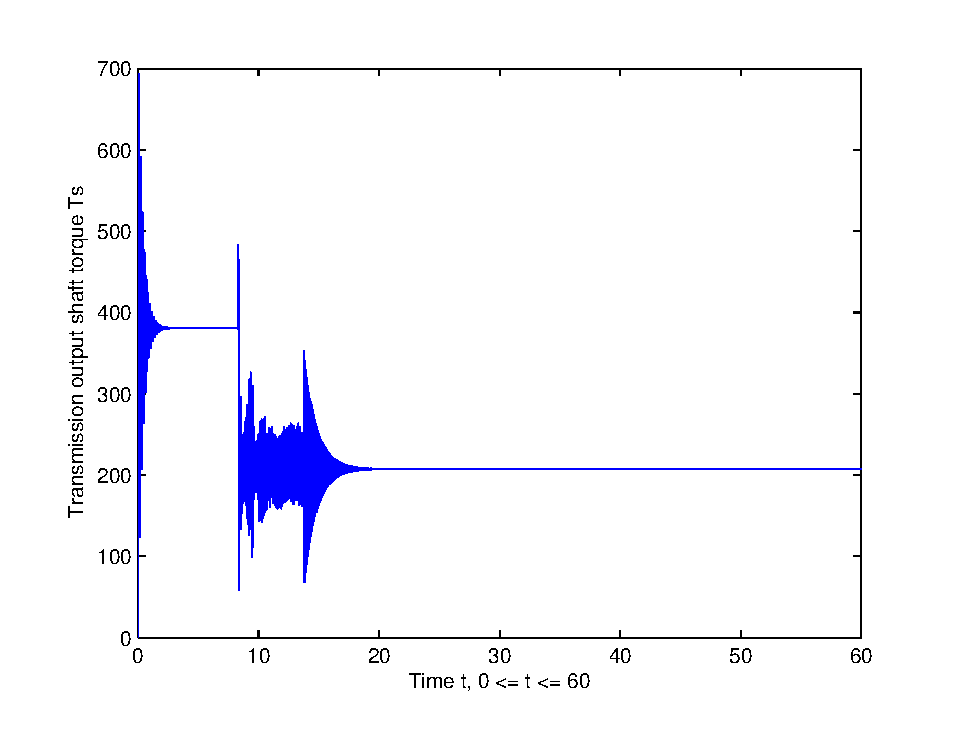
\includegraphics[angle=0,scale=0.22]{Ts-tps10-grade0} &
\includegraphics[angle=0,scale=0.22]{V-tps10-grade0} &
\includegraphics[angle=0,scale=0.22]{Gear-tps10-grade0} 
\end{tabular}

Gear change from 1st to 2nd at around 10s.
\end{slide}
%---------------------------------------------------------------------
\begin{slide}
\heading{Powertrain Simulation Plots: tps=50\%,grade=0.1}
\begin{tabular}{ccc}
Transmission Torque & Vehicle Speed & Gear
\\ \hline
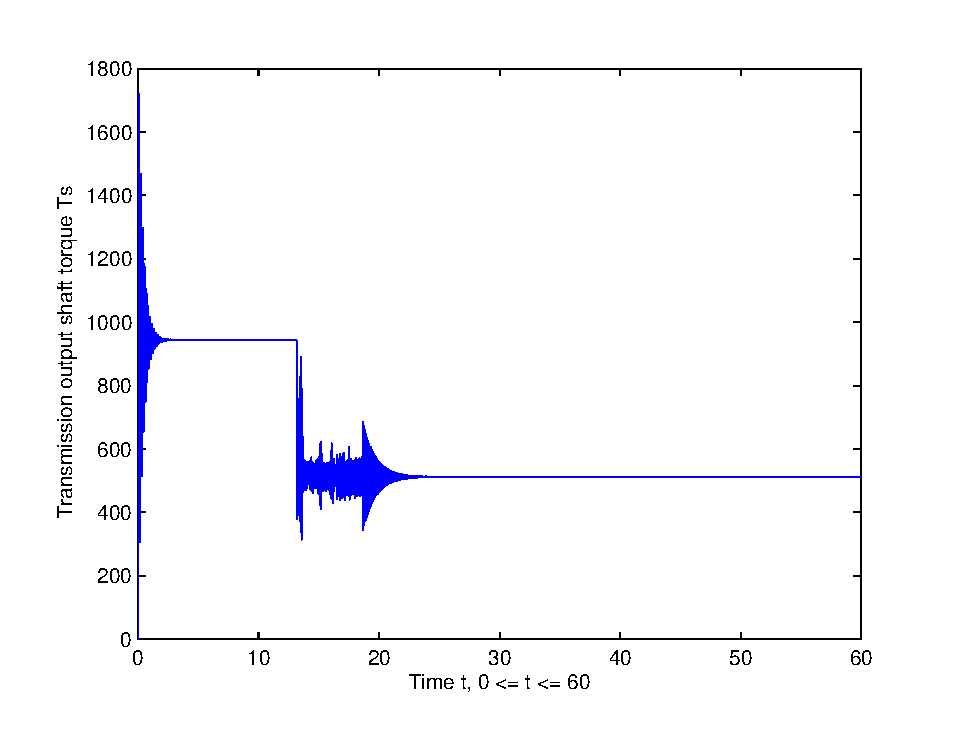
\includegraphics[angle=0,scale=0.22]{Ts-tps50-grade1} &
\includegraphics[angle=0,scale=0.22]{V-tps50-grade1} &
\includegraphics[angle=0,scale=0.22]{Gear-tps50-grade1} 
\end{tabular}

Gear change from 1st to 2nd at around 12s.
\end{slide}
%---------------------------------------------------------------------
\begin{slide}
\heading{Powertrain Simulation Plots: tps=80\%,grade=0.2}
\begin{tabular}{ccc}
Transmission Torque & Vehicle Speed & Gear
\\ \hline
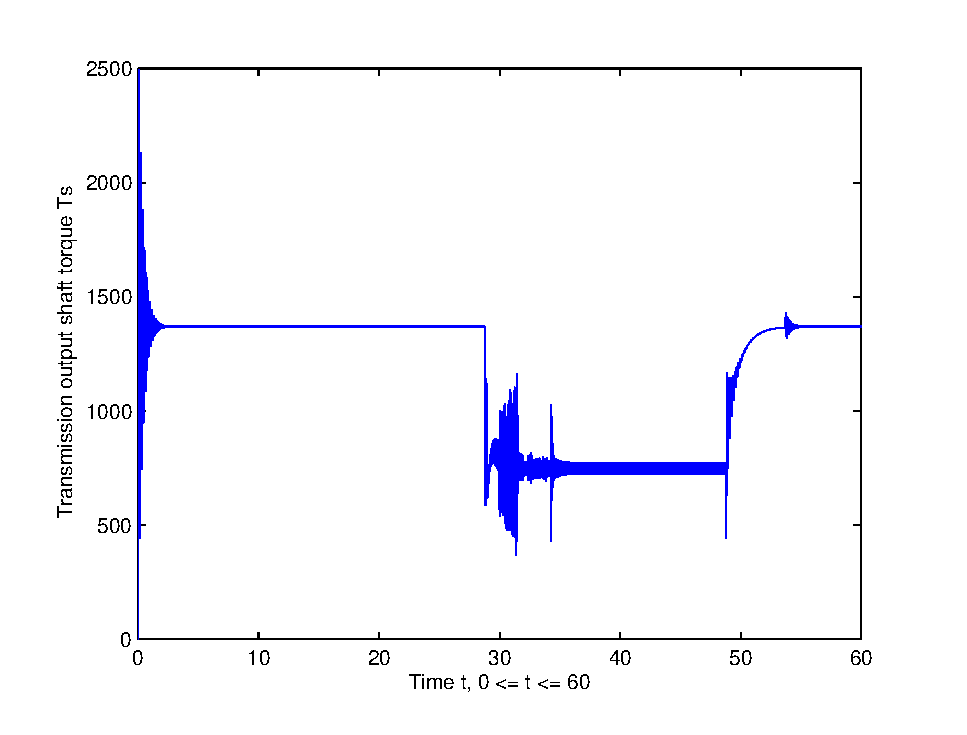
\includegraphics[angle=0,scale=0.22]{Ts-tps80-grade2} &
\includegraphics[angle=0,scale=0.22]{V-tps80-grade2} &
\includegraphics[angle=0,scale=0.22]{Gear-tps80-grade2} 
\end{tabular}

Gear change from 1st to 2nd at around 30s and 
an (incorrect) elongated back switch to 1st at 40--50s.
\end{slide}
%---------------------------------------------------------------------
\begin{slide}
\heading{Powertrain Simulation Plots: tps=80\%,grade=0.2}
\begin{tabular}{ccc}
Transmission Torque & Vehicle Speed & Gear
\\ \hline
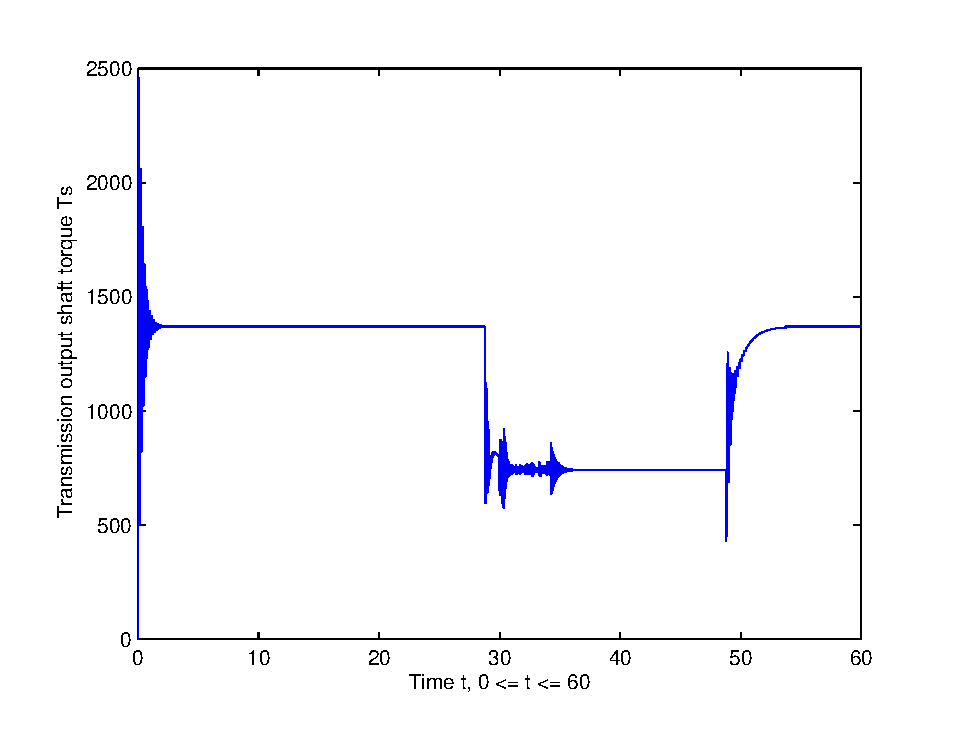
\includegraphics[angle=0,scale=0.22]{Ts-tps80-grade2-2} &
\includegraphics[angle=0,scale=0.22]{V-tps80-grade2-2} &
\includegraphics[angle=0,scale=0.22]{Gear-tps80-grade2-2} 
\end{tabular}

Gear change from 1st to 2nd at around 30s and correctly
switching back to 1st at 50+s.
\end{slide}
% -------------------------------------------------------
\end{document}
